\section{Augmented Reality in Educational Environments}

\subsection{Definition of "Augmented Reality"}
Although the term 'Augmented Reality' was coined by Tom Caudell, a former Boeing researcher, in 1990, the concept of augmenting the real world with virtual data was initially used by a number of applications in the late 1960s and 1970s. Since the 1990s, AR was used by some large companies in purpose of visualization and training. Nowerdays, the rising power of personal computers and mobile devices enable the concept of AR to be delivered to traditional educational environments such as schools and universities. \autocite [cf.][21]{Johnson.2010} 
\begin{figure}[ptbh]
    \centering
    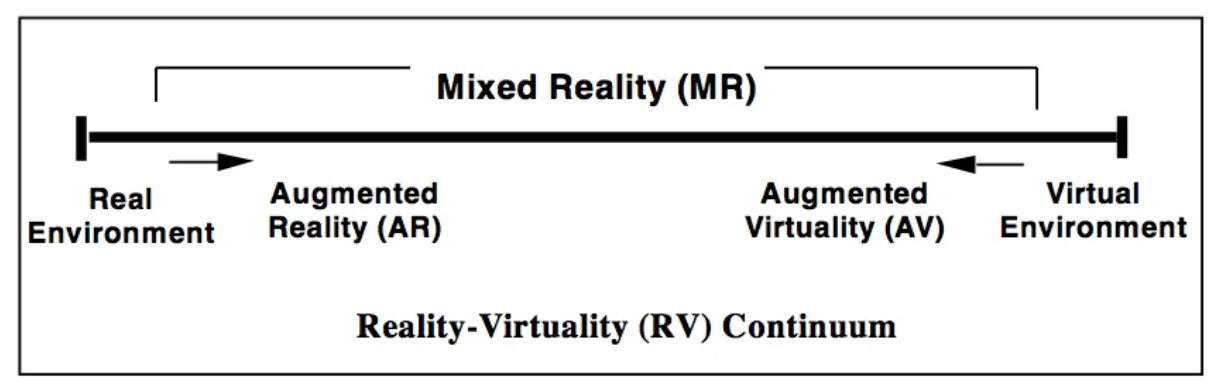
\includegraphics[width=\linewidth]{figures/rvc.png}
    \caption[Reality-Virtuality Continuum]{Reality-Virtuality Continuum}
    \label{fig:RealityVirtualityContinuum}
\end{figure}

During the last years the term 'Augmented Reality' has been given different meanings by varying researchers. \autocite [cf.][42]{Wu.2013} \cite{Milgram.1994b} defined AR on the basis of the reality-virtuality continuum (\ref{fig:RealityVirtualityContinuum}) as "augmenting natural feedback to the operator with simulated cues". \autocite[283]{Milgram.1994b} The reality-virtuality continuum (\ref{fig:RealityVirtualityContinuum}) allows us to distinguish the concept of AR to related concepts such as Virtual Reality (VR) where "the participant observer is totally immersed in a completely synthetic world" \autocite[283]{Milgram.1994b} or Augmented Virtuality (AV) where "the the primary world being experienced is in fact [...] predominantly 'virtual'"\autocite[4]{Milgram.1994} and augmented with information from the real world. In addition, \cite{Milgram.1994b} mention a more restricted definiton where AR is seen as "form of virtual reality where the participant's head-mounted display is transparent, allowing a clear view of the real world". \autocite[283]{Milgram.1994b} As suggested by educational researchers,\autocite[cf.][42]{Wu.2013} we reject the idea that the concept of AR is limited to any type of technology. Therefore, we broadly define AR referring to \cite{Klopfer.2008} as "a situation in which a real world context is dynamically overlaid with coherent location or context sensitive virtual information"\autocite[205]{Klopfer.2008} and regard it as a concept which is based on and realized by but conzeptualized beyond technology.

\subsection{Five Directions of Augmented Reality in Educational Environments}